\section{Abstract Vector Spaces}
\subsection{Motivation and Axiomatization}
In [IA I, Ch. 2], we studied the $n$-dimensional vector space $\bR^n =\{(x_1,\dots ,x_n)\mid x_i \in \bR\}$ with rows of length $n$, along with linear maps $\bR^n \to \bR^m$ with a one-to-one correspondence to the $m\times n$ matrices. When $m = n$ the bijective linear mapping $\varphi_A\colon \bR^n \to \bR^m$ is characterized by the determinant property $\det A \neq 0$, which allows you to use Cramer's rule for solving a system of linear equations associated with $\varphi_A$ and a fixed vector in $\bR^n$. If $\det A = 0$, solutions of the homogeneous linear system form a subspace in R, but as we mentioned back then, this subspace (or rather, the linear span) is an object of a different nature: if $\bR^n$ admits a basis $(1,0,\dots ,0),\dots ,(0,\dots ,0,1)$, the linear span $U\subset\bR^n$ usually does not admit a basis of this kind. This inconvenience arises from the overly concrete nature of $\bR^n$.

In fact, the properties VS1-VS8, which we actually used and will be reproduced below, are not unique to the space $\bR^n$. Consider, for example, the differential equation $d^2x/dt^2+ x = 0$ taught in schools. It is known that its general solution can be written as $x (t) = \alpha \sin t+\beta \cos t$. If $\alpha_0 ,\beta_0$ are such that $\alpha_0 \sin t + \beta_0 \cos t = 0$ for all $t$, then setting in turn $t_1=\pi /2,t_2=0$, we get $\alpha_0 = 0 =\beta_0$. This fact gives grounds to talk about the linearly independent particular solutions $\sin t, \cos t$ and the two-dimensional linear space formed by the general solutions of $d^2x/dt^2+ x = 0$ in the spirit of the following definition.

\begin{definition}
	Let $\fK$ be any field. A set $V$ of elements (called \textit{vectors}) is called a \textit{vector} (or \textit{linear}) \textit{space} over $\fK$ if it satisfies the following axioms.
	\begin{enumerate}[label=\alph*)]
		\item A binary operation $V\times V\to V$ is defined on $V$, usually denoted as addition: $(\vx, \vy) \mapsto \vx + \vy$, and it gives $V$ the structure of an Abelian group (\textit{the additive group of the space $V$}). That is:
		\begin{enumerate}
			\item[VS$_1$:]$\vx+\vy = \vy+\vx$\ (\textit{commutativity});
			\item[VS$_2$:]$(\vx+\vy)+\vz = \vx+(\vy+\vz)$\ (\textit{associativity});
			\item[VS$_3$:]There is a distinct element $\v0$ in $V$ called the \textit{zero vector} such that $\vx + 0 = \vx$ for every $\vx$ $\in V$;
			\item[VS$_4$:]For every $\vx$ $\in V$ there is an \textit{inverse} (or \textit{opposite}) vector $-\vx$ such that $\vx + (-\vx) = 0$.
		\end{enumerate}
		\item There is a set operation $(\lambda, \vx)\mapsto \lambda \vx$ defined on $\fK \times V$ called \textit{multiplication} of vectors in $V$ and \textit{scalars} in $\fK$ with the following properties:
		\begin{enumerate}
			\item[VS$_5$:]$1\cdot\vx = \vx$\ (\textit{unitary});
			\item[VS$_6$:]$(\alpha \beta)\vx = \alpha (\beta \vx)$ for all $\alpha ,\beta\in\fK, x\in V$\ (\textit{associativity}).
		\end{enumerate}
		Addition and multiplication are connected by two \textit{distributive laws}:
		\begin{enumerate}
			\item[VS$_7$:]$(\alpha + \beta)\vx = \alpha \vx + \beta x$;
			\item[VS$_8$:]$\lambda(\vx+\vy) = \lambda\vx + \lambda\vy$.
		\end{enumerate}
	\end{enumerate}
\end{definition}

Pay attention to the fact that the plus sign refers to the elements of the field $\fK$ (scalars) on the left-hand side of the equality in VS$_7$, and to vectors on the right-hand side. Strictly speaking, the addition operations in the additive group of $V$ and in the field $fK$ should be designated by different symbols (say, $\oplus$ and $+$), as well multiplication operations in $\fK \times V$ and $\fK$ (say, $\odot$ and $\cdot$). This is usually avoided because it is always clear what is being said. Nevertheless, in order to make this remark meaningful and to warn against possible errors, consider the set $V = \bR_+$ of positive real numbers. Setting $x\oplus y=xy$ (the usual multiplication in $\bR$) and $\lambda \odot x=x^\lambda$ ($x\in \bR_+$ raised to the power of $\lambda\in\bR$), we can easily verify the validity of the axioms VS$_1$-VS$_8$, so that $V$ is a vector space over $\bR$. The zero vector is $1\in\bR_+$. It is clear that in this case the usual notation $x + y = xy, \lambda x=x^\lambda$ could cause confusion.

Here is another example where other designations are more preferable. Let $V$ be a vector space over the field of complex numbers $\mathbb{C}$. We define a new vector space $\bar{V}$ with the same additive group of $V$, but another law of scalar multiplication: $(\lambda ,\vx)\mapsto \lambda \odot \vx = \bar{\lambda}\vx$, where $\bar{\lambda}$ is the complex conjugate of $\lambda$. Since $V \mapsto \bar{V}$ is an automorphism of the field $\mathbb{C}$, it is easy to verify that $\bar{V}$ is a vector space. Simultaneous consideration of $V$ and $\bar{V}$ without an icon $\odot$ (or some other symbol) would be difficult.

\begin{convention}
	The reader has probably noticed that we have denoted the vectors of the space $V$ by bold-face, lower-case letters, its elements italic lower-case letters and sometimes letters of the Greek alphabet. However, in abstract vector spaces preference will be given to bold-face; in specific examples, following this rule would be impractical, and representing a vector with an arrow at the top would be too cumbersome. With a little skill, the compromise we have adopted should not lead to misunderstandings.
\end{convention}

The definition of a vector space $V$ are followed by some direct consequences, which we will use in the future without any reference:

a) For all $\lambda\in\fK, \vx\in V$, $0\vx = \lambda\v0 = \v0$. In fact, by VS$_7$ $0\vx=(0+0)\vx =0\vx +0\vx$, whence $0\vx =\v0$. Similarly, $\lambda \v0 =\lambda(\v0+\v0)=\lambda\v0 +\lambda \v0$, i.e. $\lambda\v0 =\v0$;

b) $\lambda \vx =\v0\Rightarrow \lambda =0$ or $\vx =\v0$. If, for example, $\lambda\ne 0$, then $\vx =1\cdot\vx =(\lambda^{-1}\lambda)\vx =\lambda^{-1}(\lambda\vx)=\lambda^{-1}\v0=\v0$;

c) $(n\cdot 1)\vx =\vx +\vx +\dots +\vx$ ($n$ terms) for any positive integer $n$ and any $\vx\in V$ (the proof is by induction on $n$). It is natural to write simply $nx$ instead of $(n\cdot 1)\vx$, where $1$ is the unit of the field $\fK$. If $\fK$ is a field of finite characteristic $p$, then $p\vx =\v0$;

d) $(-1)\vx =-\vx$. Indeed, $\vx +(-1)\vx=1\vx+(-1)\vx =(1+(-1))\vx =0\vx=\v0$.

\subsection{Linear Hull (Span). Subspaces.}\label{sec:1.1-2}
Note that arranging any finite set of scalars $\lambda_i , \dots, \lambda_n \in \fK$ and vectors $\vx_1, \dots , \vx_n \in V$, we can formulate the expression
\[\lambda_1 \vx_1 + \dots + \lambda_n \vx_n =\sum_{i=1}^n \lambda_i \vx_i ,\]
called a \textit{linear combination} of the vectors $\vx_i$ with coefficients $\lambda_i$. More generally, if $I$ is a family of indices, possibly infinite, and $M = \{\vx_i\in V\mid i\in I\}$ is a subset of vectors in $V$, then it is legitimate to consider linear combinations $\sum_{i\in I}\lambda_i \vx_i$ with arbitrary coefficients $\lambda_i \in \fK$, among which, however, only a finite number are nonzero. Clearly, 
\[\lambda\Bigl(\sum \lambda_i\vx_i\Bigr)=\sum (\lambda\lambda_i)\vx_i\]
is a linear combination with coefficients $\lambda\lambda_i , i\in I$ for any scalar $\lambda \in \fK$. Similarly, the sum
\[\Bigl(\sum_{i\in I}\lambda_i\vx_i\Bigr)+\Bigl(\sum_{i\in I}\mu_i\vx_i\Bigr)=\sum_{i\in I}(\lambda_i+\mu_i)\vx_i\]
of two linear combinations with coefficients $\lambda_i ,\mu_i$ is the same linear combination of the vectors $\vx_i\in M$ with coefficients $\lambda_i +\mu_i$, among which again only a finite number are nonzero. Thus, the set $\langle M\rangle_\fK$ of all possible linear combinations of the vectors $\vx_i\in M$ is closed under the operations of vector addition and multiplication by scalars:
\[\lambda\in \fK,~{\vx,\mathbf y}\in \langle M\rangle\Rightarrow {\vx+\mathbf y} \in \langle M\rangle,~{\lambda \vx}\in \langle M\rangle.\]
We say that $\langle M\rangle$ is the \textit{linear hull(span)} of the set $M\subset V$\footnote{\textit{Translator's note}: the term ``linear span" is more common in modern literature and will be adopted throughout the rest of the book.}.

\begin{definition}
	Let $V$ be a vector space over $\fK$, $U\subset V$ its subset which is an additive subgroup of $U$ that transforms into itself under multiplication by scalars. Then the restriction to $U$ of the operations defined on $V$ gives $U$ the structure of a vector space. It is called a \textit{vector} (or \textit{linear}) \textit{subspace} of $V$.
\end{definition}

The intersection of any number of vector spaces is also a vector subspace (see the beginning of Para. 4 of \S\ref{sec:1.1-2}; it is easy exercise which is considered in [IA I] for the case of groups). We see that the linear span $\langle M\rangle$ of a system of vectors $M\subset V$ is a vector subspace of $V$, and, obviously, $\langle M\rangle$ is the smallest subspace of $V$ containing $M$. It is also said that $\langle M\rangle$ is the subspace \textit{spanned} by the vectors $x\in M$ or \textit{generated} by the vectors $x\in M$. If, from the very beginning, $M$ was a subspace, then $\langle M\rangle = M$.

We give some examples of vector spaces that will occur in the future.

\begin{example}[\textit{zero-dimensional space}]
	Over any field $\fK$ there exists a zero-dimensional (singleton) vector space $V = \{\v0\}$ with the law of multiplication by scalars $\lambda \v0 = \v0$.
\end{example}

\begin{example}[\textit{the base field $\fK$ as a one-dimensional coordinate space}]\label{ex:base-field-space}
	By the definition of $V=\fK$, the basic operation of $V$ coincide with the operations in $\fK$. If $1$ is the unit of the field $\fK$, then we can assume that $\fK = \langle 1\rangle$ is the linear span of $1$.
	
	More generally, if a field $\fK$ is an expansion of its subfield $\fB$, then $\fK$ can be regarded as a vector space over $\fB$. For example, the field of complex numbers $\bC$ is a vector space over the field of real numbers $\bR$, and $\bR$ is a vector space over the field of rational numbers $\bQ$.
\end{example}

\begin{example}[\textit{the $n$-dimensional coordinate space ${\fK}^n$}; see {[IA I, Ch. 2]}, where the field $\bR$ can be replaced by an arbitrary field $\fK$]
	For $n = 1$ we obtain the previous example. We will see soon (see \S\ref{sec:1.3}) that every subspace $U\subset {\fK}^n$ is a solution space of some homogeneous linear system.
\end{example}

\begin{example}[\textit{function spaces}]\label{ex:function-space}
	In [IA I, Ch. 1, \S4, Para. 1] we introduced the ring of functions $K^X$, which in fact is still a vector space over K (the ring $K$ must be replaced by a field). Thus, $X$ is an arbitrary set, $\fK$ is a field, and ${\fK}^X$ is the set of mappings (functions) $f: X\to \fK$, endowed with pointwise operations of addition and multiplication by scalars:
\begin{align*}
(f+g)(x) = f(x)+g(x) \text{\quad for all\quad} x\in X;\\
(\lambda f)(x) = \lambda (f(x)) \text{\quad for all\quad} \lambda\in F, x\in X.
\end{align*}
Each element $x\in X$ can be associated with the so-called delta function $\delta_x$, centered on $\{x\}$:
\[\delta_x(x) = 1, \quad \delta_x(x') = 0, \quad x\ne x'.\]
If $X = \{1, 2,\dots, n\}$, then instead of $\delta_i (j)$ we usually write $\delta_{ij}$, which is the standard notation for the Kronecker symbol. In this case, ${\fK}^X$ identified with ${\fK}^n$. Namely, the function $f$ is associated with a row vector of all its values $(f(1),f(2),\dots ,f(n))$, and the function itself is uniquely represented as a linear combination of delta functions
\[f = f(1)\delta_1 + f(2)\delta_2 + \dots + f(n)\delta_n.\]
In the case of an infinite set $X$, an analogous conclusion is meaningless, since the sums of an infinite number of vectors are not defined (unless we specifically take care of the topology).

In analysis, we most often consider real-valued functions defined on the whole real line, or on intervals $(a, b)\subset \bR$. It is easy to verify that the linear space $\bR^{(a,b)}$ contains as subspaces $\bR_{\mathrm{cont}}^{(a,b)}$ -- the space of all continuous functions, the space $\bR_{\mathrm{diff}}^{(a,b)}$ of all continuously differentiable functions, etc., as all the above properties are preserved when functions are added and multiplied by scalars.
\end{example}

\begin{example}
	Polynomials $f\in \fK [t]$ of degree $\le n-1$ form a vector space $P_n$ with the usual operations of addition and multiplication of polynomials by scalars. It should be noted that polynomials of degree equal to a fixed number $k$ do not form a linear space. However, form of degree $k$ form in $m$ variables, considered together with zero, form a vector space. 
\end{example}

\begin{example}
	Let $g(t)$ be a fixed continuous real function on the interval $[0,1]$, nonzero on some interval $J\subset [0,1]$, and $V_n (g)$ the set of functions of the form $f(t)g(t)$ where $f(t)$ is a polynomial of degree$\le n-1$. Then $P_n^g$ is a vector space contained in $\bR_{\mathrm{cont}}^J$.
\end{example}

\begin{example}[\textit{matrix spaces}]
	According to the rules of matrix calculus (see [IA I, Ch. 2]), any rectangular matrix of size $m\times n$ can be multiplied by an element of the field $\fK$ and any two can be added, resulting in a matrix of the same kind. All the axioms are satisfied, so the $m\times n$ matrices form a vector space. For $m = n$ the ring of square matrices $M_n (\fK)$, which is also a vector space over $\fK$, is called an \textit{algebra}, in accordance with the general definition that we will give in \S\ref{sec:2.2} of Chapter \ref{ch:2} and under which the objects of Examples \ref{ex:base-field-space} and \ref{ex:function-space} also fall.
	% TODO: 这句话到底是什么鬼
\end{example}

\begin{example}[Amer. Math. Monthly., Vol. 94, 1990, pp. 60-62]
	A matrix $A$ is called \textit{semimagic} (or a \textit{semimagic square}) if the sum of the coefficients in each row and each column are the same:
	\[\sum_{k=1}^n a_{ik} = \sum_{k=1}^na_{kj} = \sigma (A)\in \bQ,\quad 1\le i,j \le n.\]
	
	If, moreover, $\tr A=\sigma (A)\coloneqq \sum_{i=1}^n a_{i,n+1-i}$, the matrix $A$ is called \textit{magic} (or a \textit{magic square}).

	Magic squares have attracted attention since ancient times. We are interested in them for the fairly obvious reason that both the set of semimagic squares $\mathrm{SMag}_n (\bQ)$ and the set $\mathrm{Mag}_n (\bQ)$ of all magic squares of order $n$ are vector spaces over $\bQ$, and moreover, 
	\[\mathrm{Mag}_n(\bQ) \subset \mathrm{SMag}_n(\bQ) \subset M_n(\bQ).\]
	It is worth mentioning that we do not consider a purely combinatorial set of $n\times n$ magic squares with natural number coefficients $1, 2, \dots , n^2$. See on this subject: \textit{M. M. Postnikov}, Magic squares. Moscow: Nauka, 1964.
\end{example}
\subsection{Remarks on Geometric Interpretation.}
$V$ is called a \textit{real} (resp. \textit{complex}) vector space if $\fK =\bR$ (resp. $\fK =\bC$); scalars are then just numbers. It is these cases that are the most interesting from a practical point of view, although much of the theory does not depend on the nature of the field $\fK$.

The most natural model of a vector space is, of course, a set of directed segments emanating from a fixed point in the three-dimensional space in which we live. Multiplication of a segment by $\lambda \in \bR$ times corresponds to its extension by $\lambda > 1$ fold ($\lambda$-fold compression, for $\lambda\le 1$) and a change in the direction of the segment for negative $\lambda$'s. Addition of directed segments is carried out according to the parallelogram rule. This real vector space also coincides with the set of free geometric vectors, if we agree to consider equal two directed segments that can be combined by parallel translation.

Objects of the physical three-dimensional space $\bR_\Phi^3$ are usually represented by figures. In the case of multidimensional spaces (we will discuss dimension in \S\ref{sec:1.2}) our intuition is severely tested, yet a systematic appeal to geometric images is not only useful, but also necessary: to develop firm associations that revitalize the theory.

The unusual geometry of a vector space geometry can also be connected with the singularities of the field $\fK$. For example, if $\fK = \bC$, then a straight line over $\bC$ is a one-dimensional coordinate space $\bC^1$. Its clear geometric image is the plane of complex numbers $\bR^2$, which should not be confused with $\bC^2$. The point $(x, y) \in \bR^2$ corresponds to the number $z = x + iy\in \bC^1$; multiplication by $a\ne 0$ corresponds to stretching by a factor of $|a|$ and counterclockwise rotation by the angle $\arg a$. In particular, for $a=-1$ the restriction of the rotation of $\bC^1$ by $\ang{180}$ to $\bR^1$ gives the ``inversion" of the straight line $\bR^1$. In Chapter 3, \S4, the operations of complexification and decomplexification will be described, allowing us to take advantage of the algebraic closure of $\bC$ (for working with real vector spaces), and the $n$-dimensional complex space $\bC^n$ be represented as a $2n$-dimensional real space $\bR^{2n}$.

Note also that the physical space $\bR_\Phi^3$ is much richer than the coordinate space of the same dimension, since in $\bR_\Phi^3$ the lengths of vectors, the angles between them, and the area and volume of figures are defined. All this additional information is inadvertently transferred to figures designed to reflect the properties of abstract vector spaces, the axiomatics of which are still poor. Its enrichment with metric concepts is fully realized only in subsequent chapters.

The extent to which the vector space $V$ carries the imprint of the properties of the scalar field can also be seen from the fact that if $\fK$ is a finite field, then the geometric images introduced from $\fK^3$ are ``leaky" (a consequence of the discreteness of $\fK$). But this disadvantage of $\fK$ can sometimes be beaten (Fig.~\ref{fig:discrete-image}), by associating discrete images of a different kind with a linear geometry over $\fK$. For example, the $n$-dimensional coordinate space $\bF_2^n$ over a field of two elements $\bF_2 =\{0,1\}\cong\bZ_2$ admits a natural identification with the set $\{(\eps_1 ,\eps_2 ,\dots ,\eps_n ); \eps_i =0 \text{ or } \eps_i = 1\}$ of the vertices of the $n$-dimensional cube in $\bR^n$.

\begin{figure}
	\centering
	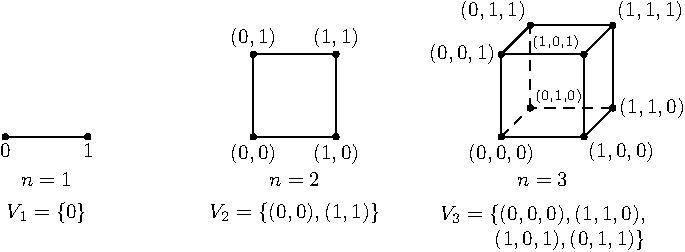
\includegraphics[width=0.8\textwidth]{../fig/fig-1.pdf}
	\caption{}
	\label{fig:discrete-image}
\end{figure}

The subspace $V_n$ consisting of points with $\eps_1 +\eps_2 + \dots + \eps_n = 0$ (recall that $1 + 0 = 0 + 1 = 1, 0 + 0 = 0 = 1 + 1$) defines the simplest code that corrects one error (see [IA I, Chapter 4, \S4, p. 7\footnote{\textit{Translator's note}: Reference is to Russian version.}]). That is, provided that the encoded signals correspond only to a point $(\eps_1 ,\eps_2 ,\dots ,\eps_n )\in V_n$ and receiving a signal $(\eps_1 ',\eps_2 ',\dots ,\eps_n ')$ with $\eps_1 +\eps_2 + \dots + \eps_n = 1$, we can reasonably assume that the transmission of this message was distorted by external interference. Of course, our code with parity check will not find two distortions, since in that case $(\eps_1 ',\eps_2 ',\cdots ,\eps_n ') \in V_n$.